\section{Graphical User Interface}
\noindent The Graphical User Interface is fully designed and implemented in Unity game engine version 5.4.1f1 Personal. Only standard unity assets are used, no additional elements are required. All of the implementation is written in C\# programming language.

\subsection{EPIC 1 Specific Info}
\noindent In EPIC 1 all of the users are gathered on the same device and all of the user actions are performed with this device's mouse and keyboard.

\subsection{Palette of colors}
\noindent The following picture shows the full spectrum of colors that are used in the project.

\begin{figure}[h]\label{gui-colors}
	\centering
	\captionsetup{justification=centering}
	\begin{subfigure}{0.105\textwidth}
		\centering
		
\includegraphics[scale=1, frame]{gui-imgs/R46G49B56A255}
		\vspace*{-20px}\caption*{\hspace*{-0.25px}\tiny R46 G49 B56 \\ \tiny A255}
	\end{subfigure}
	\begin{subfigure}{0.105\textwidth}
		\centering
		
\includegraphics[scale=1, frame]{gui-imgs/R69G73B84A64}
		\vspace*{-20px}\caption*{\hspace*{-0.25px}\tiny R69 G73 B84 \\ \tiny A64}
	\end{subfigure}
	\begin{subfigure}{0.105\textwidth}
		\centering
		
\includegraphics[scale=1, frame]{gui-imgs/R69G73B84A255}
		\vspace*{-20px}\caption*{\hspace*{-0.25px}\tiny R69 G73 B84 \\ \tiny A255}
	\end{subfigure}
 	\begin{subfigure}{0.105\textwidth}
		\centering
		
\includegraphics[scale=1, frame]{gui-imgs/R51G153B255A64}
		\vspace*{-20px} \caption*{\hspace*{-0.25px}\tiny R153 G0 B255 \\ \tiny A264}
	\end{subfigure}
	\begin{subfigure}{0.105\textwidth}
		\centering
		
\includegraphics[scale=1, frame]{gui-imgs/R255G153B102A64}
		\vspace*{-20px} \caption*{\hspace*{-0.25px}\tiny R51 G153 B255 \\ \tiny A64}
	\end{subfigure}
	\begin{subfigure}{0.105\textwidth}
		\centering
		
\includegraphics[scale=1, frame]{gui-imgs/R255G153B102A255}
		\vspace*{-20px} \caption*{\hspace*{-0.25px}\tiny R255 G153 B102 \\ \tiny A255}
	\end{subfigure} \\
 	\begin{subfigure}{0.105\textwidth}
		\centering
		
\includegraphics[scale=1, frame]{gui-imgs/R51G153B255A255}
		\vspace*{-20px} \caption*{\hspace*{-0.25px}\tiny R51 G153 B255 \\ \tiny A255}
	\end{subfigure}
	\begin{subfigure}{0.105\textwidth}
		\centering
		
\includegraphics[scale=1, frame]{gui-imgs/R153G0B255A255}
		\vspace*{-20px} \caption*{\hspace*{-0.25px}\tiny R153 G0 B255 \\ \tiny A255}
	\end{subfigure}
	\begin{subfigure}{0.105\textwidth}
		\centering
		
\includegraphics[scale=1, frame]{gui-imgs/R153G0B255A64}
		\vspace*{-20px} \caption*{\hspace*{-0.25px}\tiny R153 G0 B255 \\ \tiny A64}
	\end{subfigure}
	\begin{subfigure}{0.105\textwidth}
		\centering
		
\includegraphics[scale=1, frame]{gui-imgs/R214G0B147A64}
		\vspace*{-20px}\caption*{\hspace*{-0.25px}\tiny R214 G0 B147 \\ \tiny A64}
	\end{subfigure}
	\begin{subfigure}{0.105\textwidth}
		\centering
		
\includegraphics[scale=1, frame]{gui-imgs/R214G0B147A255}
		\vspace*{-20px} \caption*{\hspace*{-0.25px}\tiny R214 G0 B147 \\ \tiny A255}
	\end{subfigure}
	\begin{subfigure}{0.105\textwidth}
		\centering
		
\includegraphics[scale=1, frame]{gui-imgs/R0G204B153A255}
		\vspace*{-20px} \caption*{\hspace*{-0.25px}\tiny R0 G204 B153 \\ \tiny A255}
	\end{subfigure} \\
	\begin{subfigure}{0.105\textwidth}
		\centering
		
\includegraphics[scale=1, frame]{gui-imgs/R0G204B153A255}
		\vspace*{-20px} \caption*{\hspace*{-0.25px}\tiny R0 G204 B153 \\ \tiny A255}
	\end{subfigure}
	\begin{subfigure}{0.105\textwidth}
		\centering
		
\includegraphics[scale=1, frame]{gui-imgs/R102G255B102A255}
		\vspace*{-20px} \caption*{\hspace*{-0.25px}\tiny R102 G255 B102 \\ \tiny A255}
	\end{subfigure}
	\begin{subfigure}{0.105\textwidth}
		\centering
		
\includegraphics[scale=1, frame]{gui-imgs/R102G255B102A64}
		\vspace*{-20px} \caption*{\hspace*{-0.25px}\tiny R102 G255 B102 \\ \tiny A64}
	\end{subfigure}
	\begin{subfigure}{0.105\textwidth}
		\centering
		
\includegraphics[scale=1, frame]{gui-imgs/R0G204B153A64}
		\vspace*{-20px} \caption*{\hspace*{-0.25px}\tiny R255 G153 B102 \\ \tiny A64}
	\end{subfigure}
	\begin{subfigure}{0.105\textwidth}
		\centering
		
\includegraphics[scale=1, frame]{gui-imgs/R255G255B255A255}
		\vspace*{-20px}\caption*{\hspace*{-0.25px}\tiny R255 G255 B255 \\ \tiny A255}
	\end{subfigure}
	\begin{subfigure}{0.105\textwidth}
		\centering
		
\includegraphics[scale=1]{gui-imgs/R255G255B255A255}
	\end{subfigure}
	\caption{Pallete of colors}
\end{figure}

\subsection{Components}
\noindent The GUI is build with standart unity UI objects. These objects have been built into components that make up the user interface.

\subsubsection{PlayersSettingsPanel}\label{gui-playerssettingspanel}
\noindent The main GUI canvas object contains one \verb|Panel| object named \verb|PlayerSettingsPanel|. It is the user interface background on which all other components are placed. The \cprotect{\hyperref[gui-colors]}{\verb|R46 G49 B56 A255|} value is used as its color. The panel size is \verb|650x457| pixels.

\subsubsection{PlayerDisabledPanel}\label{gui-playerdisabledpanel}
\noindent One of the fundamental elements that is a part of GUI is \verb|PlayerDisabledPanel|. It's the unity \verb|Button| object which is used to add a player to the game. The component color is of value \cprotect{\hyperref[gui-colors]}{\verb|R69 G73 B84 A64)|}. It consist of two subcomponents. The first one is an inactive \verb|InputField| unity object which indicates what will be the player color after the game start. There are six player colors available: \cprotect{\hyperref[gui-colors]}{\verb|R214 G0 B147 A64)|}, \cprotect{\hyperref[gui-colors]}{\verb|R153 G0 B255 A64)|}, \cprotect{\hyperref[gui-colors]}{\verb|R51 G153 B255 A64)|},\cprotect{\hyperref[gui-colors]}{\verb|R255 G153 B102 A64)|}, \cprotect{\hyperref[gui-colors]}{\verb|R0 G204 B153 A64)|}, \cprotect{\hyperref[gui-colors]}{\verb|R102 G255 B102 A64)|}. The second one is \verb|Text| object with default \verb|+| value which indicates that PlayerDisabledPanel is to be pressed. Below pictures shows the panel details. \newpage

\begin{figure}[h!]
	\centering
	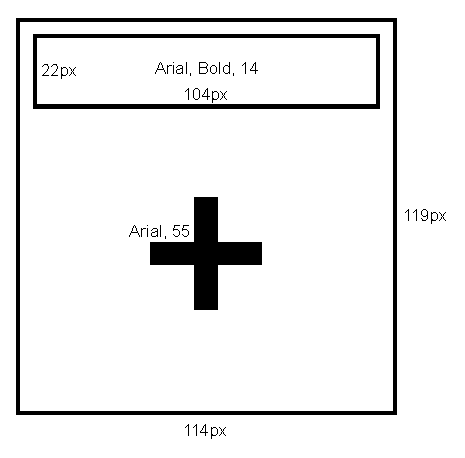
\includegraphics[scale=1]{gui-imgs/playerdisabledpanel-size}
	\caption{PlayerDisabledPanel size}
\end{figure}

\noindent The ingame pictures of all possible PlayerDisabledPanels look as follows:

\begin{figure}[h!] 
	\centering
	\begin{subfigure}{0.185\textwidth}
		\centering
		
\includegraphics[scale=1, frame]{gui-imgs/player1disabledpanel}
	\end{subfigure}
	\begin{subfigure}{0.185\textwidth}
		\centering
		
\includegraphics[scale=1, frame]{gui-imgs/player2disabledpanel}
	\end{subfigure}
	\begin{subfigure}{0.185\textwidth}
		\centering
		
\includegraphics[scale=1, frame]{gui-imgs/player3disabledpanel}
	\end{subfigure} \\
	\begin{subfigure}{0.185\textwidth}
		\centering
		
\includegraphics[scale=1, frame]{gui-imgs/player4disabledpanel}
	\end{subfigure}
	\begin{subfigure}{0.185\textwidth}
		\centering
		
\includegraphics[scale=1, frame]{gui-imgs/player5disabledpanel}
	\end{subfigure}
	\begin{subfigure}{0.185\textwidth}
		\centering
		
\includegraphics[scale=1, frame]{gui-imgs/player6disabledpanel}
	\end{subfigure}
	\caption{InGame PlayerDisabledPanels}
\end{figure}

\subsubsection{PlayerEnabledPanel}\label{gui-playerenabledpanel}
\noindent The \verb|PlayerEnabledPanel| is activated version of the \cprotect{\hyperref[gui-playerdisabledpanel]}{\verb+PlayerDisabledPanel+}. The only difference in colors is the transparency, i.e. PlayerEnabledPanel is opaque. There is on more \verb|Button| object located on InputFiled which is used to remove player from the game. Its constat \verb|X| text has the same color as the InputField. Instead of Text \verb|+| object the panel contains two more \verb|Button| objets. The buttons are used to set players movenet keys. Both Buttons are the same and have \cprotect{\hyperref[gui-colors]}{\verb|(R46 G49 B56 A255)|} color.
\newpage

\begin{figure}[h!]
	\centering
	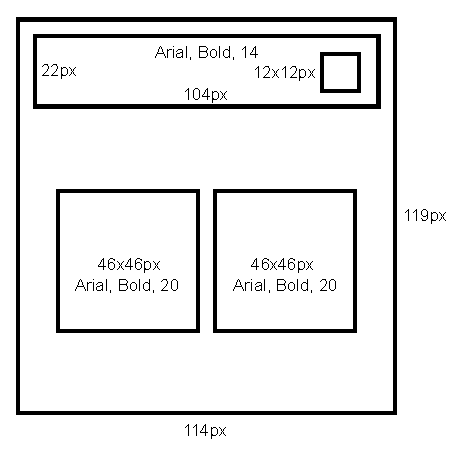
\includegraphics[scale=1]{gui-imgs/playerenabledpanel-size}
	\caption{PlayerEnabledPanel size}
\end{figure}

\noindent The ingame pictures of all possible PlayerDisabledPanels look as follows:

\begin{figure}[h!] 
	\centering
	\begin{subfigure}{0.195\textwidth}
		\centering
		
\includegraphics[scale=1, frame]{gui-imgs/player1enabledpanel}
	\end{subfigure}
	\begin{subfigure}{0.195\textwidth}
		\centering
		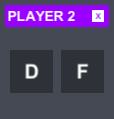
\includegraphics[scale=1, frame]{gui-imgs/player2enabledpanel}
	\end{subfigure}
	\begin{subfigure}{0.195\textwidth}
		\centering
		
\includegraphics[scale=1, frame]{gui-imgs/player3enabledpanel}
	\end{subfigure} \\
	\begin{subfigure}{0.195\textwidth}
		\centering
		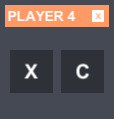
\includegraphics[scale=1, frame]{gui-imgs/player4enabledpanel}
	\end{subfigure}
	\begin{subfigure}{0.195\textwidth}
		\centering
		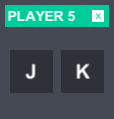
\includegraphics[scale=1, frame]{gui-imgs/player5enabledpanel}
	\end{subfigure}
	\begin{subfigure}{0.195\textwidth}
		\centering
		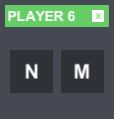
\includegraphics[scale=1, frame]{gui-imgs/player6enabledpanel}
	\end{subfigure}
	\caption{InGame PlayerEnabledPanels}
\end{figure}

\noindent All of the componetns has its default values hardcoded. All of them are explained in the \hyperref[gui-implementation]{implementation} section.

\subsubsection{ArenaSizePanel}\label{gui-arenasizepanel}
\noindent The \verb+ArenaSizePanel+ background color is exactly the same as the color of the \cprotect{\hyperref[gui-playerenabledpanel]}{\verb|PlayerEnabledPanel|}. The panel itself contains two main components. The first one is a \verb+Panel+ with the background color the same as the color of the \cprotect{\hyperref[gui-playerssettingspanel]}{\verb|PlayersSettingsPanel|}. This panel contains a "ARENA SIZE" \verb+Text+ of \cprotect{\hyperref[gui-colors]}{\verb|(R255 G255 B255 A255)|} color written in capitals letters only. The second element of the panel is a \verb+Slider+ of the following two possible colors depeneding on status: \cprotect{\hyperref[gui-colors]}{\verb|(R255 G255 B255 A255)|} in case it is not filled and \cprotect{\hyperref[gui-colors]}{\verb|(R0 G255 B153 A255)|} otherwise.
\newpage

\begin{figure}[h!]
	\centering
	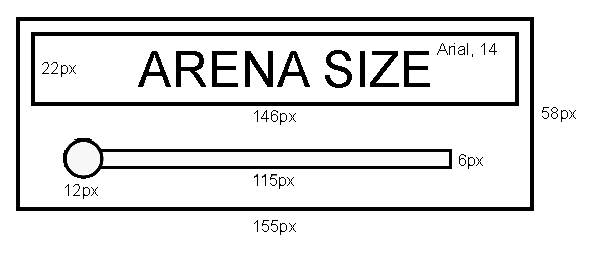
\includegraphics[scale=1]{gui-imgs/arenasizepanel-size}
	\caption{ArenaSizePanel size}
\end{figure}

\noindent The ingame pictures of the component looks as follows:

\begin{figure}[h] 
	\centering
	\begin{subfigure}{0.2\textwidth}
		\centering
		
\includegraphics[scale=1, frame]{gui-imgs/slider0}
	\end{subfigure}
	\begin{subfigure}{0.2\textwidth}
		\centering
		
\includegraphics[scale=1, frame]{gui-imgs/slider1}
	\end{subfigure}
	\caption{InGame ArenaSizePanel Slider}
\end{figure}

\begin{figure}[h!] 
	\centering
	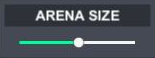
\includegraphics[scale=1, frame]{gui-imgs/arenasizepanel}
	\caption{InGame ArenaSizePanel}
\end{figure}

\noindent The functionality and implemetation of \verb+ArenaSizePanel+ is described in \hyperref[gui-implementation]{implementation} section.

\subsubsection{InitialSpeedPanel}\label{gui-initialspeedpanel}
\noindent The only differece between \verb+InitialSpeedPanel+ and \verb+ArenaSizePanel+ is the text displayed on the panel. In this case it is "PLAYERS SPEED". For detailed information about the colors and components please refer to \cprotect{\hyperref[gui-arenasizepanel]}{\verb+ArenaSizePanel+} section.

\begin{figure}[h!] 
	\centering
	
\includegraphics[scale=1, frame]{gui-imgs/initialspeedpanel}
	\caption{InGame InitialSpeedPanel}
\end{figure}

\subsubsection{InitialSizePanel}\label{gui-initialsizepanel}
\noindent The only differece between \verb+InitialSpeedPanel+ and \verb+ArenaSizePanel+ is the text displayed on the panel. In this case it is "PLAYERS SIZE". For detailed info about the colors and components please refer to \cprotect{\hyperref[gui-arenasizepanel]}{\verb+ArenaSizePanel+} section.

\begin{figure}[h!] 
	\centering
	
\includegraphics[scale=1, frame]{gui-imgs/initialsizepanel}
	\caption{InGame InitialSizePanel}
\end{figure}

\subsubsection{StartButton}\label{gui-startbutton}
\noindent The color of the "START" \verb+Button+ is the same as the color of the \hyperref[gui-arenasizepanel]{'slider panels'} text panel background. The \verb+Text+ "START" has a pure white color.
\newpage

\begin{figure}[h!] 
	\centering
	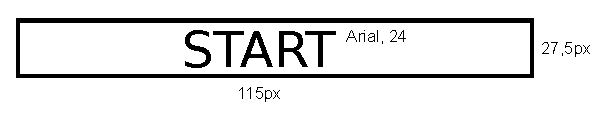
\includegraphics[scale=1]{gui-imgs/startbutton-size}
	\caption{StartButton size}
\end{figure}

\noindent The ingame pictures of the component looks as follows:

\begin{figure}[h!]
	\centering
	
\includegraphics[scale=1, frame]{gui-imgs/startbutton}
	\caption{InGame StartButton}
\end{figure}

\subsubsection{Startup GUI}
\noindent Here is an example of a GUI just after the game starts:

\begin{figure}[h!] 
	\centering
	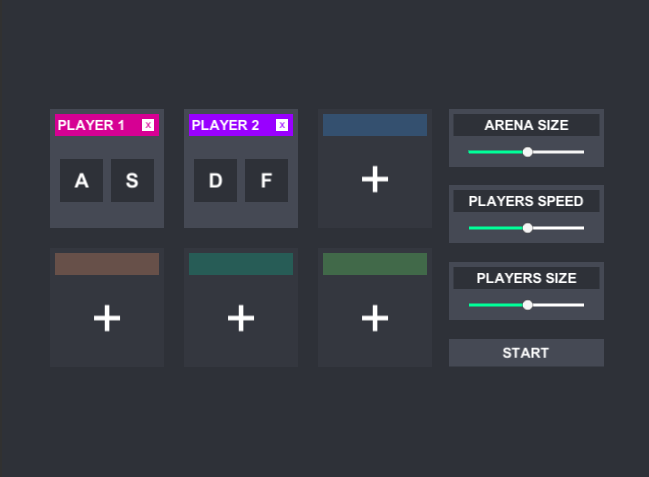
\includegraphics[width=\textwidth, frame]{gui-imgs/startupgui}
	\caption{Startup GUI}
\end{figure}


\subsection{Implemetation}\label{gui-implementation}
\indent The GUI implementation is located in \textit{GUIManager.cs} script which uses \textit{GUIHelper.cs} that contains helpful methods. The file is using \textit{Configurator.cs} script to write the user settings before game starts. The following functionalities are implemented:

\begin{itemize}
	\item[-] Reading initial game configuration. It is stored in 'default.cfg' file.
	\item[-] Adding and Removing player. There is a minimum of two players that must participate the game. There is no possibility  to lower the value from the GUI. A user can manipulate the number of players from two to six. It is also impossible to have more than six players in the game.
	\item[-] Setting the nickname of the player. On each \cprotect{\hyperref[gui-playerenabledpanel]}{\verb+PlayerEnabledPanel+} there is an \verb+InputField+ by witch user can set player unique name. The nickname is limited by 9 characters and may contain only english alphabet letters and digit.
	\item[-] Setting the player movement keys. Each player must have its own movement keys. There is no possibility that two playes has the Setting key set. There is also no possibility that the player has the same key set for both directions.
	\item[-] Changing the initial arena size. The \cprotect{\hyperref[gui-arenasizepanel]}{\verb+ArenaSizePanel+} slider allows user to set the initial arena size. There are three possible sizes of the arena: small, normal and big.
	\item[-] Setting the initial speed of all players. The \cprotect{\hyperref[gui-initialspeedpanel]}{\verb+InitialSpeedPanel+} slider allows user to set the initial speed value. There are three possible speeds to be set: slow, normal and fast.
	\item[-] Setting the initial size of all players. The \cprotect{\hyperref[gui-initialsizepanel]}{\verb+InitialSizePanel+} slider allows user to set the initial size value. There are three possible sizes to be set: thin, normal and fat.
	\item[-] Starting the game. The \cprotect{\hyperref[gui-startbutton]}{\verb+StartButton+} loads a new scene with the game itself.
\end{itemize} 

\subsection{Sounds}
\indent There are no sounds implemented on the GUI yet.